%%%%%%%%%%%%%%%%%%%%%%%%%%%%%%%%%%%%%%%%%%%
%%%%%%%%%%%%%%%%%%%%%%%%%%%%%%%%%%%%%%%%%%%
%%%%%%%%%%%%%%% CHAPTER 10 %%%%%%%%%%%%%%%%


\section{Análise da resposta transitória e de regime permanente}

\frame{
\frametitle{Introdução}
\begin{block}{Contextualização}
Em capítulos anteriores, foi dito que o primeiro passo para a análise de um sistema de controle é a obtenção de um \textbf{modelo matemático} do sistema. Uma vez obtido esse modelo, é possível analisar o \textbf{desempenho do sistema} a partir dos vários métodos disponíveis.
\end{block}
}

\frame{
\frametitle{Introdução}
\begin{block}{Sinais de testes}
Na análise e no projeto de sistemas de controle, devemos ter uma \textbf{base de comparação} do desempenho de vários sistemas de controle.
\begin{itemize}
    \item Essa base pode ser estabelecida detalhando-se \textbf{sinais de entrada de teste} específicos e, em seguida, \textbf{comparando-se} as respostas dos vários sistemas com esses sinais.
\end{itemize}
\end{block}
}

\frame{
\frametitle{Introdução}
\begin{block}{Sinais de testes}
Os sinais de entrada de teste geralmente utilizados são as funções:
\begin{itemize}
    \item degrau;
    \item rampa;
    \item parábola;
    \item impulso;
    \item senoidal;
    \item ruído branco.
\end{itemize}
\vspace{0.5cm}
Com esses sinais de teste, tanto a análise \textbf{experimental} como a análise \textbf{matemática} dos sistemas de controle podem ser obtidas facilmente, uma vez que esses sinais são funções de tempo \textbf{muito simples}.
\end{block}
}

\frame{
\frametitle{Introdução}
\begin{block}{Sinais de testes - qual utilizar?}
Deve-se escolher de acordo com o \textbf{comportamento da entrada} a que o sistema será submetido.
\begin{itemize}
    \item Se as entradas de um sistema de controle são funções de tempo que variam \textbf{gradualmente}, então a \textbf{rampa} em função do tempo pode ser um bom sinal de teste.
    \item Da mesma maneira, se um sistema estiver sujeito a variações \textbf{bruscas} de entrada, a função \textbf{degrau} poderá ser um bom sinal de teste.
    \item Da mesma forma, se o sistema estiver sujeito a entradas de \textbf{impacto}, uma função \textbf{impulso} poderá ser a melhor opção.
\end{itemize}
\end{block}
}

\frame{
\frametitle{Resposta transitória e resposta estacionária}
\begin{block}{Definição}
A resposta temporal de um sistema de controle consiste em duas partes: a resposta \textbf{transitória} e a resposta \textbf{estacionária}.
\begin{itemize}
    \item Resposta transitória (resposta natural): aquela que vai do estado inicial ao estado final.
    \item Resposta estacionária (resposta em regime permanente ou resposta forçada): comportamento do sinal de saída do sistema na medida em que $t$ tende ao infinito.
\end{itemize}
$$c(t) = c_{tr}(t) + c_{ss}(t)$$
\end{block}
}

\frame{
\frametitle{Polos e zeros de um sistema}
\begin{block}{Polos de uma função de transferência}
Os \textbf{polos} de uma função de transferência são
\begin{enumerate}
    \item os valores da variável da transformada de Laplace, $s$, que fazem com que a função de transferência se torne \textbf{infinita}, ou
    \item quaisquer raízes do denominador da função de transferência que são comuns às raízes do numerador.
\end{enumerate}
\end{block}
}

\frame{
\frametitle{Polos e zeros de um sistema}
\begin{block}{Zeros de uma função de transferência}
Os \textbf{zeros} de uma função de transferência são
\begin{enumerate}
    \item os valores da variável da transformada de Laplace, $s$, que fazem com que a função de transferência se torne \textbf{zero}, ou
    \item quaisquer raízes do numerador da função de transferência que são comuns às raízes do denominador.
\end{enumerate}
\end{block}
}

\frame{
\frametitle{Exemplo $\#01$ - Polos e zeros de um sistema}
\centerline{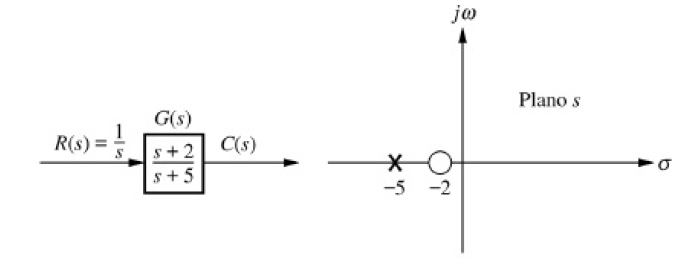
\includegraphics[width=0.9\linewidth]{Figuras/Ch10/fig1.PNG}}
\begin{block}{}
Considerando a função de transferência $G(s)$ acima, existe um \textbf{polo} em $s=-5$ e um \textbf{zero} em $s=-2$. Esses valores são representados \textbf{graficamente} no plano $s$ complexo.
\end{block}
}

\frame{
\frametitle{Exemplo $\#01$ - Polos e zeros de um sistema}
\begin{block}{}
Vamos agora determinar a reposta do sistema quando submetido a um degrau unitário.
$$C(s) = \dfrac{(s+2)}{s(s+5)} = \dfrac{A}{s} + \dfrac{B}{s+5} = \dfrac{2/5}{s} + \dfrac{3/5}{s+5}$$
Deste modo,
$$c(t) = \dfrac{2}{5} + \dfrac{3}{5}e^{-5t}$$
\end{block}
}

\frame{
\frametitle{Exemplo $\#01$ - Polos e zeros de um sistema}
\begin{block}{Conclusões}
\begin{itemize}
    \item Um polo da função de entrada gera a forma da \textit{resposta forçada} (isto é, o polo na origem gerou uma função degrau na saída).
    \item Um polo da função de transferência gera a forma da \textit{resposta natural} (isto é, o polo em $-5$ gerou $e^{-5t}$).
    \item Um polo no eixo real gera uma resposta \textit{exponencial} da forma $e^{-\alpha t}$, em que $-\alpha$ é a posição do polo no eixo real. Assim, quanto mais à esquerda um polo estiver no eixo real negativo, mais rápido a resposta transitória exponencial decairá para zero.
    \item Os zeros e os polos geram as \textit{amplitudes} para ambas as respostas, forçada e natural.
\end{itemize}
\end{block}
}

\frame{
\frametitle{Exemplo $\#02$ - Polos e zeros de um sistema}
\centerline{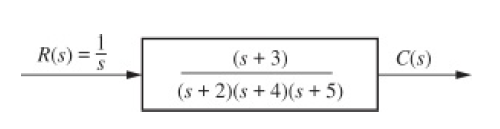
\includegraphics[width=0.6\linewidth]{Figuras/Ch10/fig2.PNG}}
\begin{block}{}
Dado o sistema acima, escreva a saída, $c(t)$, em termos gerais. Especifique as partes forçada e natural da solução. \\
\vspace{0.5cm}
\textbf{Resolução:}
$$C(s) = \underbrace{\dfrac{A}{s}}_{\text{\tiny Resposta forçada}} + \underbrace{\dfrac{B}{s+2} + \dfrac{C}{s+4} + \dfrac{D}{s+5}}_{\text{\tiny Resposta natural}}$$
Aplicando a transformada inversa de Laplace, obtemos
$$c(t) = \underbrace{A}_{\text{\tiny Resposta forçada}} + \underbrace{Be^{-2t} + Ce^{-4t} + De^{-5t}}_{\text{\tiny Resposta natural}}$$
\end{block}
}

\frame{
\frametitle{Sistemas de primeira ordem}
\centerline{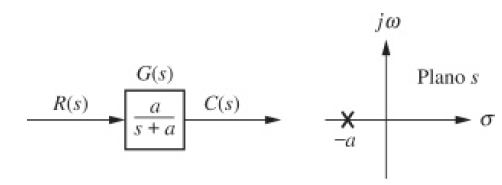
\includegraphics[width=0.7\linewidth]{Figuras/Ch10/fig3.PNG}}
\begin{block}{Introdução}
Um sistema de primeira ordem \textbf{sem zeros} pode ser descrito pela função de transferência mostrada na figura acima.
\begin{itemize}
    \item Caso a entrada seja um degrau unitário, temos que:
\end{itemize}
$$C(s) = \dfrac{a}{s(s+a)} \implies c(t) = 1 - e^{-at}$$
\end{block}
}

\frame{
\frametitle{Sistemas de primeira ordem - especificações de desempenho}
\begin{block}{Constante de tempo}
Chamamos $1/a$ a \textbf{constante de tempo} da resposta.
$$c(t) = 1 - e^{-at} \ \therefore \ c(1/a) = 1 - e^{-1} = 1 - 0,37 = 0,63$$
Deste modo, a constante de tempo é o \textbf{tempo necessário para a resposta do degrau atingir 63\% de seu valor final}.
\begin{itemize}
    \item Uma vez que o polo da função de transferência está em $-a$, podemos dizer que o polo está localizado no \textit{inverso} da constante de tempo, e \textbf{quanto mais afastado o polo estiver do eixo imaginário, mais rápida será a resposta transitória}.
\end{itemize}
\end{block}
}

\frame{
\frametitle{Sistemas de primeira ordem - especificações de desempenho}
\centerline{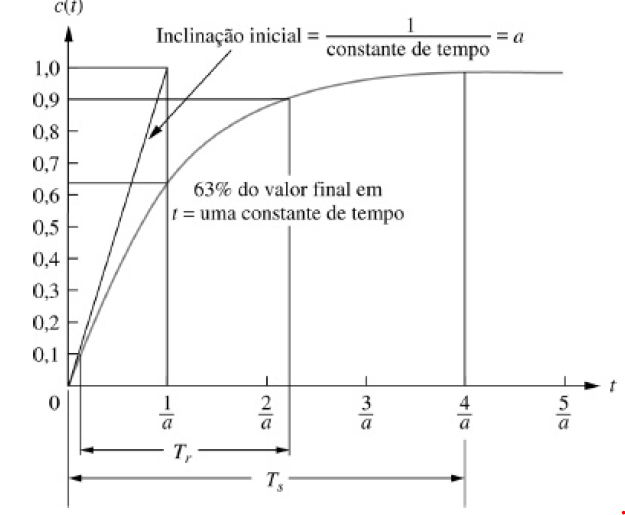
\includegraphics[width=0.7\linewidth]{Figuras/Ch10/fig4.PNG}}
}

\frame{
\frametitle{Sistemas de primeira ordem - especificações de desempenho}
\begin{block}{Tempo de subida}
O \textbf{tempo de subida} ($T_r$) é definido como o \textbf{tempo necessário para que a forma de onda vá de 0,1 a 0,9 de seu valor final.}
$$c(t) = 1 - e^{-at} \ \therefore \ 0,9 = 1 - e^{-at} \implies 0,1 = e^{-at} \implies t \approx \dfrac{2,3}{a}$$
$$c(t) = 1 - e^{-at} \ \therefore \ 0,1 = 1 - e^{-at} \implies 0,9 = e^{-at} \implies t \approx \dfrac{0,1}{a}$$
Deste modo,
$$\boxed{T_r = \dfrac{2,3}{a} - \dfrac{0,1}{a} = \dfrac{2,2}{a}}$$
\end{block}
}

\frame{
\frametitle{Sistemas de primeira ordem - especificações de desempenho}
\begin{block}{Tempo de acomodação}
O \textbf{tempo de acomodação} ($T_s$) é definido como o \textbf{tempo para que a resposta alcance e fique em uma faixa de 2\% em torno do seu valor final.}
$$c(t) = 1 - e^{-at} \ \therefore \ 0,98 = 1 - e^{-at} \implies 0,02 = e^{-at} \implies t \approx \dfrac{4}{a}$$
Deste modo,
$$\boxed{T_s = \dfrac{4}{a}}$$
\end{block}
}

\frame{
\frametitle{Exemplo $\#03$ - sistema de primeira ordem}
\begin{block}{}
Um sistema possui uma função de transferência $G(s) = \dfrac{50}{s+50}$. \\ Determine $T$, $T_r$ e $T_s$. \\
\vspace{0.5cm}
\textbf{Resolução:}
$$G(s) = \dfrac{50}{s+50} = \dfrac{a}{s+a}$$
Deste modo, $a = 50$. Com isso,
\vspace{0.3cm}
\begin{itemize}
    \item $T = \dfrac{1}{a} = \dfrac{1}{50} = \SI{0,02}{\second}$.
    \vspace{0.3cm}
    \item $T_r = \dfrac{2,2}{a} = \dfrac{2,2}{50} = \SI{0,044}{\second}$.
    \vspace{0.3cm}
    \item $T_s = \dfrac{4}{a} = \dfrac{4}{50} = \SI{0,08}{\second}$.
\end{itemize}
\end{block}
}

\frame{
\frametitle{Exemplo $\#04$ - sistema de primeira ordem a partir de ensaios}
\centerline{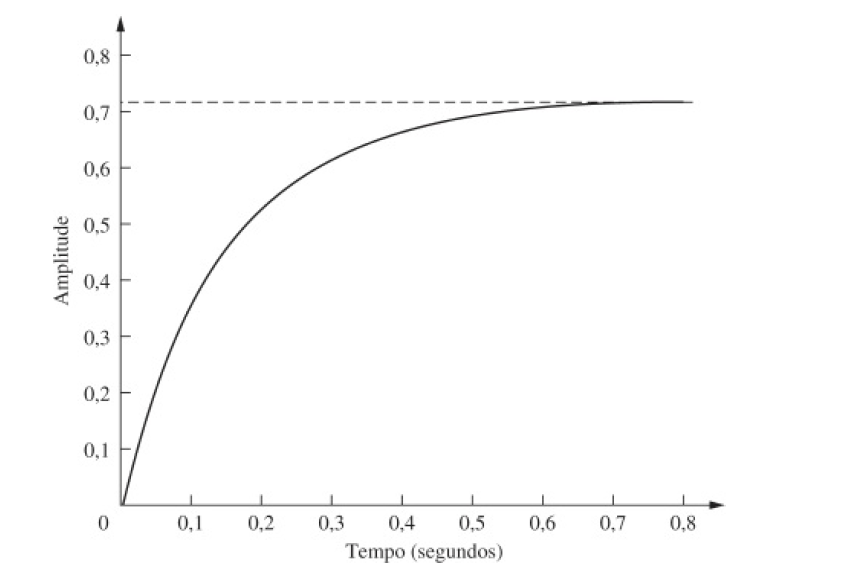
\includegraphics[width=0.75\linewidth]{Figuras/Ch10/fig5.PNG}}
\begin{block}{}
Considere a resposta ao degrau de um sistema de primeira ordem simples mostrada acima. Determine a função de transferência aproximada.
\end{block}
}

\frame{
\frametitle{Exemplo $\#04$ - sistema de primeira ordem a partir de ensaios}
\begin{block}{Resolução}
$$C(s) = \dfrac{K}{s(s+a)} = \dfrac{K/a}{s} - \dfrac{K/a}{(s+a)}$$
\begin{itemize}
    \item Como o valor final é aproximadamente 0,72, a constante de tempo é determinada onde a curva atinge $0,63 \times 0,72 = 0,4536$, o que dá aproximadamente $\SI{0,13}{\second}$. Deste modo, $a = 1/0,13 \approx 7,7$.
    \item A resposta forçada atinge um valor em regime permanente de $K/a = 0,72 \implies K \approx 5,54$.
\end{itemize}
\vspace{0.2cm}
Com isso,
$$G(s) = \dfrac{5,54}{s+7,7}$$
\end{block}
}

\frame{
\frametitle{Sistemas de segunda ordem}
\begin{block}{Introdução}
\begin{itemize}
    \item Um sistema de segunda ordem exibe uma \textbf{ampla variedade de respostas} que devem ser analisadas e descritas.
    \item A variação de um parâmetro em um sistema de segunda ordem, além de alterar a velocidade da resposta (assim como em sistemas de primeira ordem), modifica também a \textbf{forma da resposta}.
\end{itemize}
\end{block}
}

\frame{
\frametitle{Sistemas de segunda ordem - ideia intuitiva}
\begin{block}{Respostas transitórias de segunda ordem possíveis}
Considere um sistema de segunda ordem do tipo 
$$G(s) = \dfrac{b}{s^2 + as + b}$$
Podemos perceber a presença de dois polos finitos e nenhum zero.
\begin{itemize}
    \item Atribuindo valores apropriados aos parâmetros $a$ e $b$, podemos mostrar todas as \textbf{respostas transitórias de segunda ordem possíveis}, considerando o degrau unitário como entrada.
\end{itemize}
\end{block}
}

\frame{
\frametitle{Sistemas de segunda ordem - ideia intuitiva}
\centerline{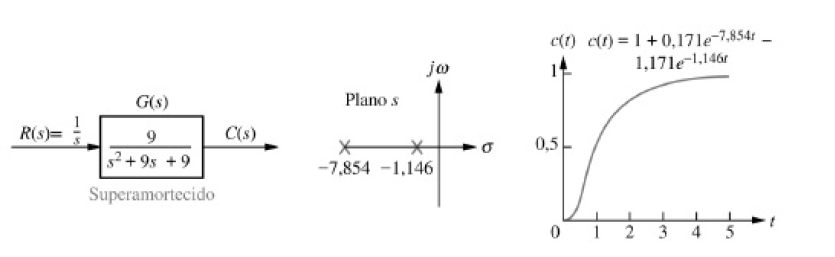
\includegraphics[width=1\linewidth]{Figuras/Ch10/fig6.PNG}}
\begin{block}{Resposta superamortecida}
$$C(s) = \dfrac{9}{s(s^2 + 9s + 9)} = \dfrac{9}{s(s+7,854)(s+1,146)}$$
\begin{itemize}
    \item Polos: dois reais em $-\sigma_1$ e $-\sigma_2$
    \item Resposta natural: $c(t) = K_1e^{-\sigma_1t} + K_2e^{-\sigma_2t}$
\end{itemize}
\end{block}
}

\frame{
\frametitle{Sistemas de segunda ordem - ideia intuitiva}
\centerline{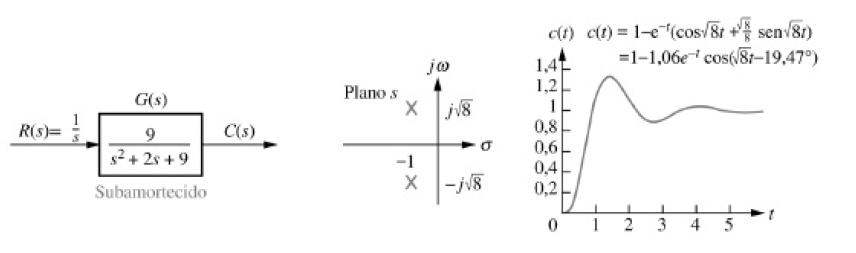
\includegraphics[width=1\linewidth]{Figuras/Ch10/fig7.PNG}}
\begin{block}{Resposta subamortecida}
$$C(s) = \dfrac{9}{s(s^2 + 2s + 9)} = \dfrac{9}{s(s+1-j\sqrt{8})(s+1+j\sqrt{8})}$$
\begin{itemize}
    \item Polos: dois complexos em $-\sigma_d \pm j\omega_d$
    \item Resposta natural: $c(t) = Ae^{-\sigma_dt} cos(\omega_d t - \phi)$
\end{itemize}
\end{block}
}

\frame{
\frametitle{Sistemas de segunda ordem - ideia intuitiva}
\centerline{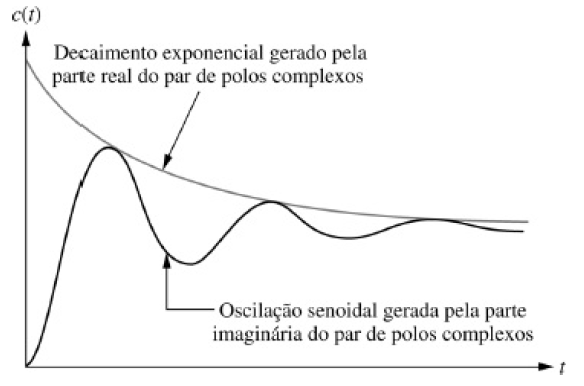
\includegraphics[width=0.6\linewidth]{Figuras/Ch10/fig8.PNG}}
}

\frame{
\frametitle{Sistemas de segunda ordem - ideia intuitiva}
\centerline{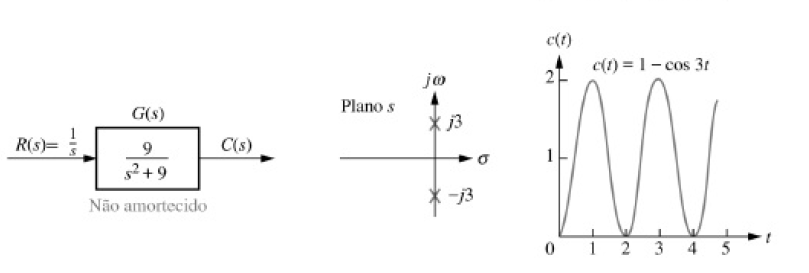
\includegraphics[width=1\linewidth]{Figuras/Ch10/fig9.PNG}}
\begin{block}{Resposta não amortecida (oscialação sustentada)}
$$C(s) = \dfrac{9}{s(s^2 + 9)} = \dfrac{9}{s(s-j3)(s+j3)}$$
\begin{itemize}
    \item Polos: dois imaginários em $\pm j\omega_1$
    \item Resposta natural: $c(t) = Acos(\omega_1 t - \phi)$
\end{itemize}
\end{block}
}

\frame{
\frametitle{Sistemas de segunda ordem - ideia intuitiva}
\centerline{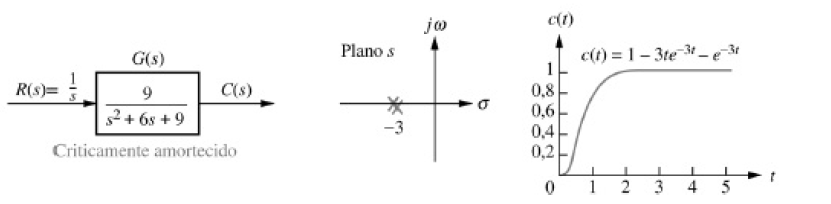
\includegraphics[width=1\linewidth]{Figuras/Ch10/fig10.PNG}}
\begin{block}{Resposta criticamente amortecida}
$$C(s) = \dfrac{9}{s(s^2 + 6s + 9)} = \dfrac{9}{s(s+3)^2}$$
\begin{itemize}
    \item Polos: dois reais em $-\sigma_1$
    \item Resposta natural: $c(t) = K_1e^{-\sigma_1t} + K_2te^{-\sigma_1t}$ 
\end{itemize}
\end{block}
}

\frame{
\frametitle{Sistemas de segunda ordem - ideia intuitiva}
\centerline{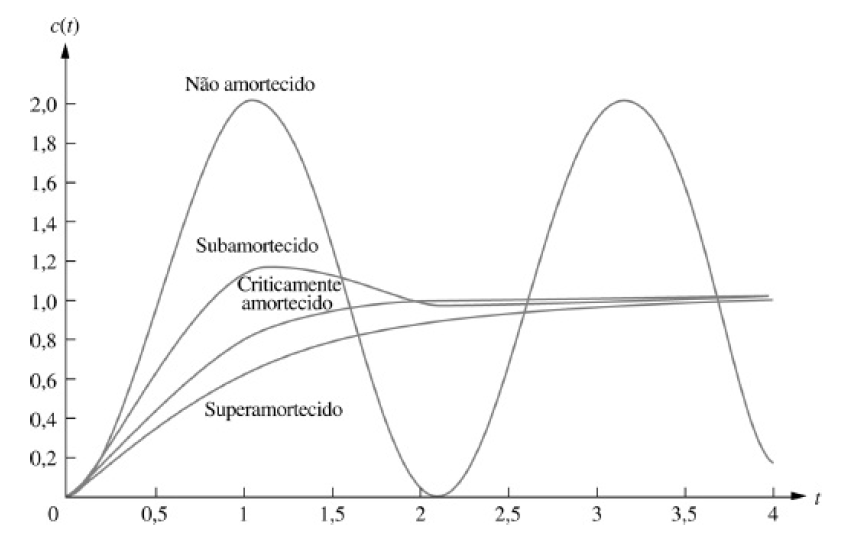
\includegraphics[width=0.7\linewidth]{Figuras/Ch10/fig11.PNG}}
\begin{block}{Em resumo...}
\begin{itemize}
    \item Observe que o caso \textbf{criticamente amortecido} é o divisor entre os casos superamortecidos e os casos subamortecidos, e é a \textbf{resposta mais rápida sem ultrapassagem}. 
\end{itemize}
\end{block}
}

\frame{
\frametitle{O sistema de segunda ordem geral}
\begin{block}{Grandezas}
\begin{itemize}
    \item A \textbf{frequência natural} ($\omega_n$) de um sistema de segunda ordem é a frequência de oscilação do sistema \textbf{sem amortecimento}.
    \item Uma definição viável para o \textbf{coeficiente de amortecimento} ($\zeta$) é aquela que considera a \textbf{razão} entre a frequência de decaimento exponencial da envoltória e a frequência natural. Essa razão é constante, independente da escala de tempo da resposta.
\end{itemize}
\end{block}
}

\frame{
\frametitle{O sistema de segunda ordem geral}
\begin{block}{Sistema geral}
$$G(s) = \dfrac{b}{s^2 + as + b}$$
\begin{itemize}
    \item Obtenção de $b$:
\end{itemize}
Sem amortecimento, os polos estariam no eixo $j\omega$, e a resposta seria uma senoide não amortecida. Para que os polos sejam imaginários puros, $a=0$. Portanto,
$$G(s) = \dfrac{b}{s^2 + b}$$
Como os polos estão localizados em $\pm j\sqrt{b}$, temos que
$$\omega_n = \sqrt{b} \ \therefore \ \boxed{b = \omega_n^2}$$
\end{block}
}

\frame{
\frametitle{O sistema de segunda ordem geral}
\begin{block}{Sistema geral}
$$G(s) = \dfrac{b}{s^2 + as + b}$$
\begin{itemize}
    \item Obtenção de $a$:
\end{itemize}
Admitindo um sistema subamortecido, os polos complexos possuem uma parte real, $\sigma$, igual a $-a/2$. A magnitude desse valor é então a frequência de decaimento exponencial. Portanto,
$$\zeta = \dfrac{a/2}{\omega_n}$$
Deste modo,
$$\boxed{a = 2 \zeta \omega_n}$$
\end{block}
}

\frame{
\frametitle{O sistema de segunda ordem geral}
\begin{block}{Sistema geral}
Nossa função de transferência de segunda ordem geral, finalmente, apresenta a forma:
$$\boxed{G(s) = \dfrac{\omega_n^2}{s^2 + 2 \zeta \omega_n s + \omega_n^2}}$$
\begin{itemize}
    \item Calculando os polos da função de transferência, resulta
\end{itemize}
$$s_{1,2} = -\zeta \omega_n \pm \underbrace{\omega_n\sqrt{\zeta^2-1}}_{\omega_d}$$
\end{block}
}

\frame{
\frametitle{O sistema de segunda ordem geral}
\centerline{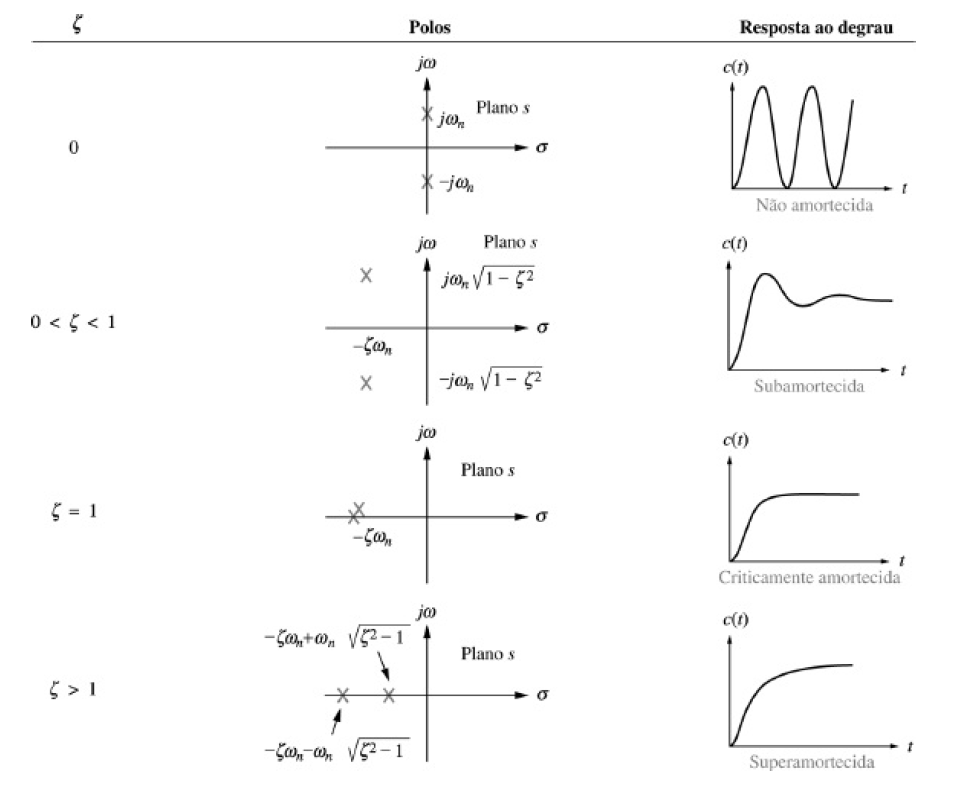
\includegraphics[width=0.8\linewidth]{Figuras/Ch10/fig12.PNG}}
}

\frame{
\frametitle{Sistemas de segunda ordem subamortecidos}
\begin{block}{Resposta ao degrau}
$$C(s) = \dfrac{\omega_n^2}{s(s^2+2\zeta \omega_n s + \omega_n^2)} = \dfrac{\omega_n^2}{(s+ \zeta \omega_n)^2 + \omega_d^2} \cdot \dfrac{1}{s}$$
pois, tem-se:
$$(s+ \zeta \omega_n)^2 = s^2 + 2s\zeta \omega_n + \zeta^2\omega_n^2$$
$$(s+ \zeta \omega_n)^2 - \zeta^2\omega_n^2 = s^2 + 2s\zeta \omega_n$$
$$(s+ \zeta \omega_n)^2 \underbrace{-\zeta^2\omega_n^2 + \omega_n^2}_{\omega_d^2} = s^2 + 2s\zeta \omega_n + \omega_n^2$$
$$(s+ \zeta \omega_n)^2  + \omega_d^2 = s^2 + 2s\zeta \omega_n + \omega_n^2$$
Utilizando-se frações parciais, tem-se:
$$C(s) = \dfrac{1}{s} - \dfrac{s + \zeta \omega_n}{(s+ \zeta \omega_n)^2 + \omega_d^2} - \dfrac{\zeta \omega_n}{(s+ \zeta \omega_n)^2 + \omega_d^2}$$
\end{block}
}

\frame{
\frametitle{Sistemas de segunda ordem subamortecidos}
\begin{block}{Resposta ao degrau}
$$C(s) = \dfrac{1}{s} - \dfrac{s + \zeta \omega_n}{(s+ \zeta \omega_n)^2 + \omega_d^2} - \dfrac{\Bigg(\dfrac{\zeta}{\sqrt{1-\zeta^2}}\Bigg)\omega_d}{(s+ \zeta \omega_n)^2 + \omega_d^2}$$
Deste modo,
$$c(t) = 1 - e^{-\zeta \omega_n t}cos(\omega_d t) - \dfrac{\zeta}{\sqrt{1-\zeta^2}}e^{-\zeta \omega_n t}sen(\omega_d t)$$
$$c(t) = 1 - e^{-\zeta \omega_n t}\Bigg(cos(\omega_d t) + \dfrac{\zeta}{\sqrt{1-\zeta^2}}sen(\omega_d t)\Bigg)$$
$$\boxed{c(t) = 1 - \dfrac{e^{-\zeta \omega_n t}}{\sqrt{1-\zeta^2}}sen(\omega_d t + \theta)} \ \text{em que} \ \theta = tan^{-1} \Big(\dfrac{\sqrt{1-\zeta^2}}{\zeta}\Big)$$
\end{block}
}

\frame{
\frametitle{Sistemas de segunda ordem subamortecidos}
\begin{block}{Sistema geral}
Um gráfico da resposta ao degrau do sistema de segunda ordem subamortecido é mostrado abaixo.
\begin{itemize}
    \item Perceba que quanto \textbf{menor} o valor de $\zeta$, \textbf{mais oscilatória} é a resposta.
\end{itemize}
\end{block}
\centerline{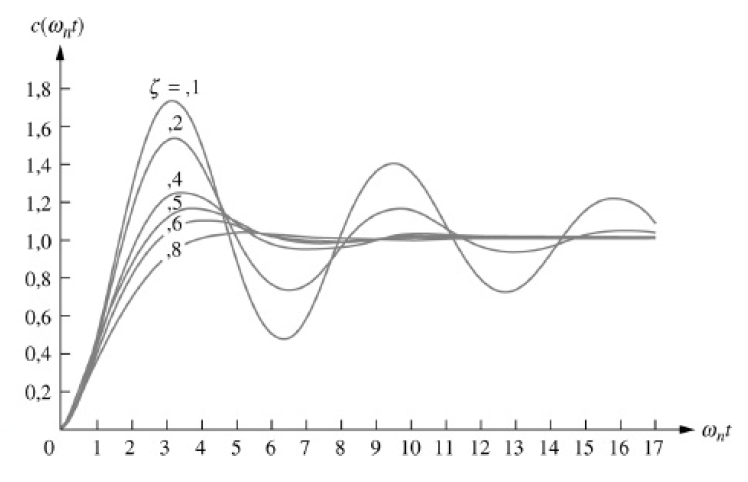
\includegraphics[width=0.6\linewidth]{Figuras/Ch10/fig13.PNG}}
}

\frame{
\frametitle{Sistemas de segunda ordem subamortecidos - especificações de desempenho}
\centerline{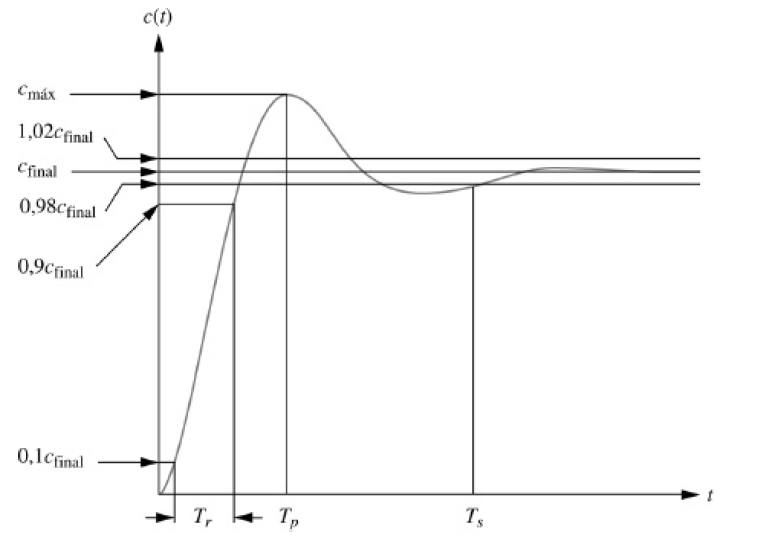
\includegraphics[width=0.85\linewidth]{Figuras/Ch10/fig14.PNG}}
}

\frame{
\frametitle{Sistemas de segunda ordem subamortecidos - especificações de desempenho}
\begin{block}{Tempo de pico}
O \textbf{tempo de pico} ($T_p$) é definido como o \textbf{tempo para que a resposta atinja o primeiro pico de sobressinal}. Pode ser obtido derivando $c(t)$ em relação a $t$ e igualando o resultado a zero:
\begin{equation*}
\begin{split}
\dfrac{dc}{dt} = \zeta \omega_n e^{-\zeta \omega_n t} \Big(cos \ \omega_d t + \dfrac{\zeta}{\sqrt{1-\zeta^2}}sen \ \omega_d t\Big) \\
+ e^{-\zeta \omega_n t} \Big(\omega_d sen \ \omega_d t - \dfrac{\zeta \omega_d}{\sqrt{1-\zeta^2}}cos \ \omega_d t\Big)
\end{split}
\end{equation*}
Simplificando e igualando a zero, obtemos:
$$\dfrac{dc}{dt} = \omega_n e^{-\zeta \omega_n t} \Big(\sqrt{1-\zeta^2} + \dfrac{\zeta^2}{\sqrt{1-\zeta^2}}\Big)sen \ \omega_d t = 0$$
\end{block}
}

\frame{
\frametitle{Sistemas de segunda ordem subamortecidos - especificações de desempenho}
\begin{block}{Tempo de pico}
Substituindo $t$ por $T_p$, temos:
$$\dfrac{dc}{dt}\Big|_{t=T_p} = (sen \ \omega_d T_p) \dfrac{\omega_n}{\sqrt{1-\zeta^2}} e^{-\zeta \omega_n T_p} = 0$$
Dessa última equação resulta a seguinte expressão:
$$sen \ \omega_d T_p = 0 \implies \omega_d T_p = 0, \pi, 2\pi, 3\pi, ...$$
Como o tempo de pico corresponde ao primeiro pico do sobressinal, $\omega_d T_p = \pi$. Então:
$$\boxed{T_p = \dfrac{\pi}{\omega_d}}$$
\end{block}
}

\frame{
\frametitle{Sistemas de segunda ordem subamortecidos - especificações de desempenho}
\begin{block}{Máximo sobressinal (\textit{overshoot})}
O \textbf{máximo sobressinal} ($M_p$) é definido como o \textbf{valor máximo de pico da curva de resposta, medido a partir da unidade}. Pode ser obtido substituindo $t = T_p$ em $c(t)$:
$$c(t) = 1 - e^{-\zeta \omega_n(\pi/\omega_d)}\Bigg(cos(\pi) + \dfrac{\zeta}{\sqrt{1-\zeta^2}}sen(\pi)\Bigg) = e^{-\zeta \omega_n(\pi/\omega_d)}$$
Então:
$$\boxed{M_p = \text{exp} \ \Bigg(\dfrac{-\zeta \pi}{\sqrt{1-\zeta^2}}\Bigg)}$$
\end{block}
}

\frame{
\frametitle{Sistemas de segunda ordem subamortecidos - especificações de desempenho}
\begin{block}{Máximo sobressinal (\textit{overshoot})}
Se o valor da resposta em regime diferir da
unidade, utiliza-se a \textbf{porcentagem máxima de sobressinal} (ou ultrapassagem
percentual, U.P.):
$$\text{U.P.} = \dfrac{c(T_p) - c(\infty)}{c(\infty)} \times 100\%$$
\begin{itemize}
    \item Caso o \textit{overshoot} $M_p$ seja conhecido, e deseja-se calcular $\zeta$, então deve-se empregar a fórmula:
\end{itemize}
$$\boxed{\zeta = \dfrac{-\text{ln}(M_p)}{\sqrt{\pi^2 + \text{ln}^2 (M_p)}}}$$
\end{block}
}

\frame{
\frametitle{Sistemas de segunda ordem subamortecidos - especificações de desempenho}
\begin{block}{Tempo de acomodação (ou assentamento)}
O \textbf{tempo de acomodação} ($T_s$) é definido como o \textbf{tempo necessário para que a resposta permaneça com valores no interior de uma certa faixa} $\pm \Delta$ (usualmente $\pm 2\%$ ou $\pm 5\%$) em torno do valor final. $$c(t) = 1 - \dfrac{e^{-\zeta \omega_n t}}{\sqrt{1-\zeta^2}}sen(\omega_d t + \theta)$$
$$\dfrac{e^{-\zeta \omega_n t}}{\sqrt{1-\zeta^2}} = 0,02$$
Esta equação é uma estimativa conservadora, uma vez que estamos admitindo $sen(\omega_d t + \theta) = 1$ no instante referente ao tempo de acomodação.
\end{block}
}

\frame{
\frametitle{Sistemas de segunda ordem subamortecidos - especificações de desempenho}
\begin{block}{Tempo de acomodação (ou assentamento)}
Resolvendo para $t = T_s$ temos:
$$T_s = \dfrac{-\text{ln}(0,02\sqrt{1-\zeta^2})}{\zeta \omega_n}$$
O numerador da equação acima varia de 3,91 até 4,74 à medida que $\zeta$ varia de 0 até 0,9. Comumente, adota-se uma aproximação dada por:
$$\boxed{T_s = \dfrac{4}{\zeta \omega_n}}$$
\end{block}
}

\frame{
\frametitle{Sistemas de segunda ordem subamortecidos - especificações de desempenho}
\begin{block}{Tempo de subida}
O \textbf{tempo de subida} ($T_r$) é definido como o \textbf{tempo requerido para que a resposta passe de $0\%$ a $100\%$} (podendo ser utilizado de $10\%$ a $90\%$). 
$$c(T_r) = 1 = 1 - e^{-\zeta \omega_n T_r}\Bigg(cos(\omega_d T_r) + \dfrac{\zeta}{\sqrt{1-\zeta^2}}sen(\omega_d T_r)\Bigg)$$
\begin{itemize}
    \item Como $e^{-\zeta \omega_n T_r} \neq 0 \implies cos(\omega_d T_r) + \dfrac{\zeta}{\sqrt{1-\zeta^2}}sen(\omega_d T_r) = 0$
\end{itemize}
$$\dfrac{cos \ \omega_d T_r}{sen \ \omega_d T_r} = - \dfrac{\zeta}{\sqrt{1-\zeta^2}} \implies tg \ \omega_d T_r = -\dfrac{\sqrt{1-\zeta^2}}{\zeta}$$
\end{block}
}

\frame{
\frametitle{Sistemas de segunda ordem subamortecidos - especificações de desempenho}
\begin{block}{Tempo de subida}
Manipulando, temos:
$$tg \ \omega_d T_r = -\dfrac{\omega_n\sqrt{1-\zeta^2}}{\zeta \omega_n}\implies \omega_d T_r = tg^{-1}\Big(-\dfrac{\omega_d}{\zeta \omega_n}\Big)$$
Deste modo,
$$T_r = \dfrac{1}{\omega_d}tg^{-1}\Big(-\dfrac{\omega_d}{\zeta \omega_n}\Big) \ \therefore \ \boxed{T_r = \dfrac{\pi - \theta}{\omega_d}}$$
\end{block}
\centerline{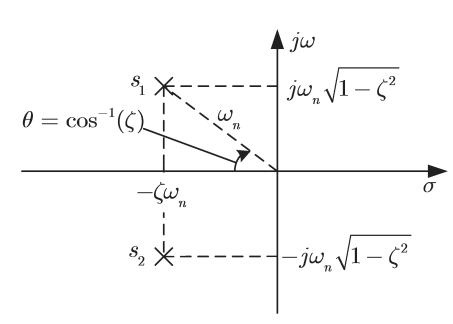
\includegraphics[width=0.4\linewidth]{Figuras/Ch10/fig15.PNG}}
}

\frame{
\frametitle{Sistemas de segunda ordem subamortecidos - especificações de desempenho}
\begin{block}{Considerações de projeto}
\begin{itemize}
    \item Deseja-se geralmente que a \textbf{resposta transitória seja rápida e amortecida}.
    \item Para um sistema de 2a ordem com \textbf{resposta transitória aceitável}, deve-se fazer $0,4 < \zeta < 0,8$.
    \item Valores \textbf{pequenos} ($\zeta < 0,4$) resultam em \textbf{excessivo sobressinal} na resposta transitória.
    \item Para valores \textbf{grandes} ($\zeta > 0,8$) a resposta se torna \textbf{muito lenta}.
    \item \textbf{Sobressinal e tempo de subida são conflitantes entre si}, ou seja, eles não
    podem ser diminuídos simultaneamente.
\end{itemize}
\end{block}
}

\frame{
\frametitle{Exemplo $\#05$ - sistema de segunda ordem subamortecido}
\begin{block}{}
Dada a função de transferência 
$$G(s) = \dfrac{100}{s^2+15s+100}$$ 
determine
\begin{itemize}
    \item $\omega_n$
    \item $\zeta$
    \item $\omega_d$
    \item $T_p$
    \item $M_p$
    \item $T_s$
    \item $T_r$
\end{itemize}
\end{block}
}

\frame{
\frametitle{Exemplo $\#05$ - sistema de segunda ordem subamortecido}
\begin{block}{Resolução}
$$G(s) = \dfrac{100}{s^2+15s+100} = \dfrac{\omega_n^2}{s^2 + 2 \zeta \omega_n s + \omega_n^2}$$ 
\begin{itemize}
    \item Por inspeção, $\omega_n = 10$ rad/s.
    \item $2\zeta \omega_n = 15 \ \therefore \ \zeta = 0,75$.
    \item $\omega_d = \omega_n \sqrt{1-\zeta^2} = 10\sqrt{1-0,75^2} = 6,61$ rad/s.
    \item $T_p = \dfrac{\pi}{\omega_d} = \dfrac{\pi}{6,61} = 0,475$ s.
    \item $M_p = \text{exp} \ \Big(\dfrac{-\zeta \pi}{\sqrt{1-\zeta^2}}\Big) = \text{exp} \ \Big(\dfrac{-0,75 \pi}{\sqrt{1-0,75^2}}\Big) = 0,0283 = 2,83\%$
    \item $T_s = \dfrac{4}{\zeta \omega_n} = \dfrac{4}{0,75 \cdot 10} = 0,533$ s.
    \item $T_r = \dfrac{\pi - \theta}{\omega_d} = \dfrac{\pi - tg^{-1}(\omega_d/\zeta \omega_n)}{\omega_d} = \dfrac{\pi - tg^{-1}(6,61/7,5)}{6,61} = 0,366$ s.
\end{itemize}
\end{block}
}

\frame{
\frametitle{Exemplo $\#06$ - sistema de segunda ordem subamortecido}
\begin{block}{}
Considerando o sistema de controle abaixo, deseja-se escolher o ganho $K$ e o
parâmetro $p$ de modo que as seguintes especificações da resposta transitória a
um degrau sejam alcançadas:
\begin{itemize}
    \item máximo \textit{overshoot} percentual igual ou inferior a $4,3\%$;
    \item tempo de assentamento para uma faixa de $2\%$ do valor final deve ser inferior a 4 s.
\end{itemize}
\end{block}
\vspace{0.2cm}
\centerline{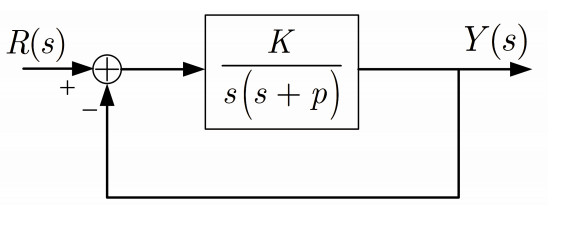
\includegraphics[width=0.6\linewidth]{Figuras/Ch10/fig16.PNG}}
}

\frame{
\frametitle{Exemplo $\#06$ - sistema de segunda ordem subamortecido}
\begin{block}{Resolução}
Considerando as especificações, temos:
\begin{itemize}
    \item máximo \textit{overshoot} percentual igual ou inferior a $4,3\%$
\end{itemize}
$$\zeta = \dfrac{-\text{ln}(M_p)}{\sqrt{\pi^2 + \text{ln}^2 (M_p)}} = \dfrac{-\text{ln}(0,043)}{\sqrt{\pi^2 + \text{ln}^2 (0,043)}} = 0,707$$
\begin{itemize}
    \item tempo de assentamento para uma faixa de $2\%$ do valor final deve ser inferior a 4 s.
\end{itemize}
Para $T_s = 4$ s, temos $T_s = \dfrac{4}{\zeta \omega_n} \implies 4 = \dfrac{4}{0,707 \omega_n} \ \therefore \ \omega_n = 1,41$ rad/s.
Deste modo,
$$\dfrac{Y(s)}{R(s)} = \dfrac{K}{s^2 + ps + K} = \dfrac{\omega_n^2}{s^2 + 2 \zeta \omega_n s + \omega_n^2} = \dfrac{2}{s^2 + 2s + 2}$$
Daí, $K = 2$ e $p = 2$.
\end{block}
}

\frame{
\frametitle{Relação entre as especificações de desempenho e a posição dos polos}
\centerline{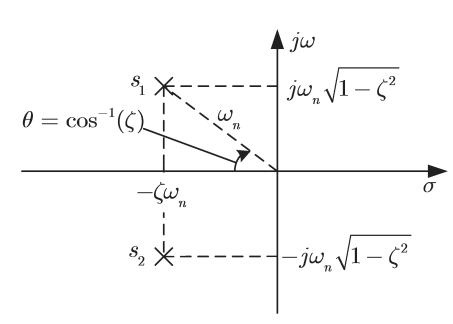
\includegraphics[width=0.7\linewidth]{Figuras/Ch10/fig15.PNG}}
}

\frame{
\frametitle{Relação entre as especificações de desempenho e a posição dos polos}
\centerline{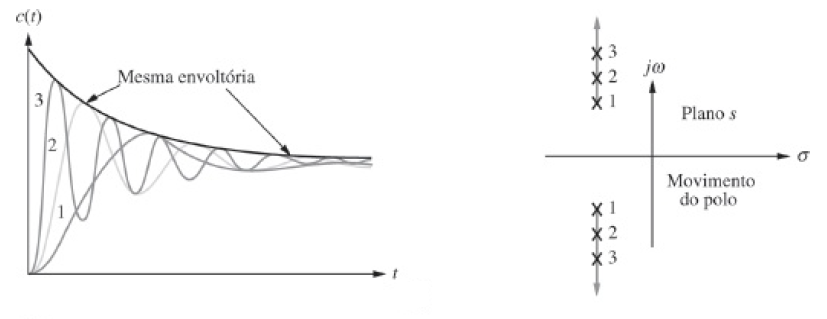
\includegraphics[width=0.9\linewidth]{Figuras/Ch10/fig17.PNG}}
\begin{block}{Polos se movendo com parte real constante}
\begin{itemize}
    \item Lembrando que $T_s = \dfrac{4}{\zeta \omega_n}$, podemos ver que $T_s$ é inversamente proporcional à parte real do polo.
    \item Uma vez que as linhas verticais no plano $s$ são linhas de valor real constante, elas também são \textbf{linhas de tempo de acomodação constante}.
\end{itemize}
\end{block}
}

\frame{
\frametitle{Relação entre as especificações de desempenho e a posição dos polos}
\centerline{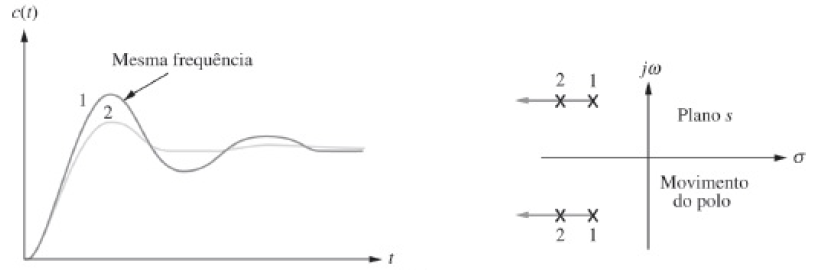
\includegraphics[width=0.95\linewidth]{Figuras/Ch10/fig18.PNG}}
\begin{block}{Polos se movendo com parte imaginária constante}
\begin{itemize}
    \item Lembrando que $T_p = \dfrac{\pi}{\omega_d}$, podemos ver que $T_p$ é inversamente proporcional à parte imaginária do polo.
    \item Uma vez que as linhas horizontais no plano $s$ são linhas de valor imaginário constante, elas também são \textbf{linhas de instante de pico constante}.
\end{itemize}
\end{block}
}

\frame{
\frametitle{Relação entre as especificações de desempenho e a posição dos polos}
\centerline{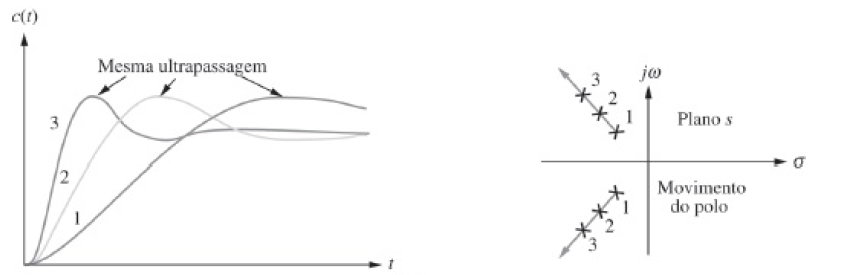
\includegraphics[width=0.95\linewidth]{Figuras/Ch10/fig19.PNG}}
\begin{block}{Polos se movendo com fator de amortecimento constante}
\begin{itemize}
    \item Lembrando que $\zeta = cos \ \theta$, linhas radiais são linhas de $\zeta$ constante.
    \item Uma vez que a ultrapassagem percentual é uma função de apenas $\zeta$, as \textbf{linhas radiais são linhas de ultrapassagem percentual constante}.
\end{itemize}
\end{block}
}

\frame{
\frametitle{Exemplo $\#07$ - sistema de segunda ordem subamortecido}
\begin{block}{}
Sendo um sistema de 2a ordem com a localização dos polos abaixo, determine $T_p$, $M_p$ e $T_s$.
\end{block}
\vspace{0.2cm}
\centerline{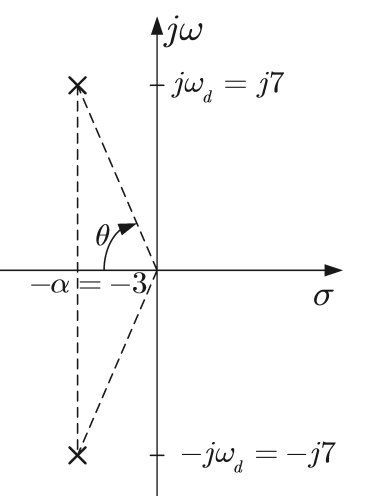
\includegraphics[width=0.4\linewidth]{Figuras/Ch10/fig20.PNG}}
}

\frame{
\frametitle{Exemplo $\#07$ - sistema de segunda ordem subamortecido}
\begin{block}{Resolução}
O fator de amortecimento é dado por:
$$\zeta = cos \ \theta = cos[tg^{-1}(7/3)] = 0,394$$
A frequência natural é a distância radial da origem ao polo, isto é, 
$$\omega_n = \sqrt{7^2+3^2} = 7,616 \ \text{rad/s}$$. 
\begin{itemize}
    \item $T_p = \dfrac{\pi}{\omega_d} = \dfrac{\pi}{7} = 0,449$ s.
    \item $M_p = \text{exp} \ \Big(\dfrac{-\zeta \pi}{\sqrt{1-\zeta^2}}\Big) = \text{exp} \ \Big(\dfrac{-0,394 \pi}{\sqrt{1-0,394^2}}\Big) = 0,26 = 26\%$
    \item $T_s = \dfrac{4}{\zeta \omega_n} = \dfrac{4}{3} = 1,333$ s.
\end{itemize}
\end{block}
}

\frame{
\frametitle{Exercícios}
\begin{block}{}
01. Determine $\zeta, \omega_n, T_s, T_p, T_r \ \text{e} \ M_p$ para um sistema cuja função de transferência é
$$G(s) = \dfrac{361}{s^2 + 16s + 361}$$

\vspace{0.5cm}

02. Dado o sistema mostrado na figura abaixo, determine $J$ e $D$ para resultar em uma ultrapassagem de $20\%$ e em um tempo de acomodação de 2 segundos, para uma entrada em degrau do torque $T(t)$.
\end{block}
\vspace{0.3cm}
\centerline{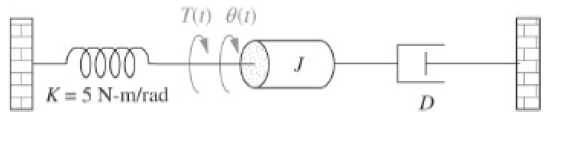
\includegraphics[width=0.8\linewidth]{Figuras/Ch10/fig21.PNG}}
}

\frame{
\frametitle{Referências e exercícios complementares}
\begin{itemize}
\item NISE, Norman S. Engenharia de Sistemas de Controle, 7 ed. LTC, 2017.
\end{itemize}
\centering{\alert{Página 172 - \textbf{Capítulo 4}}} \\
\vspace{0.4cm}
\begin{itemize}
\item OGATA, Katsuhiko. Engenharia de Controle Moderno, 5 ed. Pearson, 2010.
\end{itemize}
\centering{\alert{Página 238 - \textbf{Capítulo 5}}} \\
}